\documentclass[aspectratio=169]{beamer}

\usetheme{default}
\usecolortheme{dove}

\setbeamertemplate{navigation symbols}{}
\setbeamertemplate{footline}{%
  \hfill{\large\insertframenumber\,/\,\inserttotalframenumber}\hspace{0.8em}\vspace{0.5em}%
}

\definecolor{popblue}{RGB}{52, 101, 164}
\definecolor{sampred}{RGB}{204, 0, 0}
\definecolor{paramgreen}{RGB}{0, 140, 70}
\definecolor{warnred}{RGB}{180, 40, 40}
\definecolor{orange1}{RGB}{220, 120, 0}
\definecolor{violet1}{RGB}{120, 50, 160}
\definecolor{lightbg}{RGB}{245, 245, 250}

\setbeamercolor{frametitle}{fg=popblue}
\setbeamercolor{title}{fg=popblue}

\usepackage{pgfplots}
\usepackage{tikz}
\usetikzlibrary{shapes, arrows.meta, positioning, calc, decorations.pathreplacing, patterns}
\pgfplotsset{compat=1.18}
\usepackage{amsmath, amssymb}
\usepackage{fontenc}

\title{Information Theory II: ML Connections}
\subtitle{KL = MLE $\cdot$ Cross-Entropy Loss $\cdot$ Forward/Reverse KL $\cdot$ Mutual Information}
\date{}

\begin{document}

% ============================================================
\begin{frame}
\titlepage
\end{frame}

% ============================================================
\begin{frame}
\frametitle{Recap: The Three Pillars}

\begin{center}
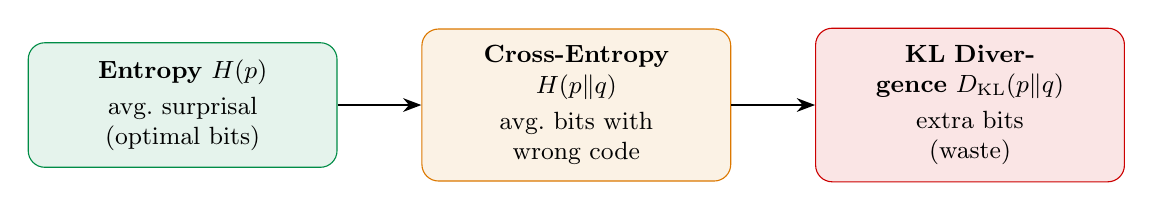
\begin{tikzpicture}[
  box/.style={draw=#1, fill=#1!10, rounded corners=6pt, minimum height=1cm, text width=3.5cm, align=center, font=\small, inner sep=6pt},
]
  \node[box=paramgreen] (ent) at (-5, 0.5) {\textbf{Entropy} $H(p)$\\[2pt]avg.\ surprisal\\(optimal bits)};
  \node[box=orange1] (ce)  at (0, 0.5) {\textbf{Cross-Entropy} $H(p\|q)$\\[2pt]avg.\ bits with\\wrong code};
  \node[box=sampred] (kl)  at (5, 0.5) {\textbf{KL Divergence} $D_{\text{KL}}(p\|q)$\\[2pt]extra bits\\(waste)};
  \draw[-{Stealth}, thick] (ent) -- (ce);
  \draw[-{Stealth}, thick] (ce) -- (kl);
\end{tikzpicture}
\end{center}

\vspace{0.1cm}
$$H(p \| q) = H(p) + D_{\text{KL}}(p \| q)$$

\vspace{0.1cm}
\begin{center}
\fcolorbox{popblue}{popblue!5}{\parbox{11cm}{\centering\small
  \textbf{Today:} We connect these concepts to machine learning.\\
  KL $\to$ MLE, \;cross-entropy $\to$ log-loss, \;forward/reverse KL,\\
  maximum entropy principle, and mutual information.
}}
\end{center}
\end{frame}

% ============================================================
\section{KL and Maximum Likelihood}

\begin{frame}
\begin{center}
\vspace{1cm}
{\LARGE\bfseries\textcolor{popblue}{KL = Maximum Likelihood}}\\[15pt]
{\large The single most important connection between}\\[4pt]
{\large information theory and machine learning.}
\end{center}
\end{frame}

% ============================================================
\begin{frame}
\frametitle{Minimizing KL = Maximizing Log-Likelihood}

\small
Data from true $p$, model family $q_\theta$. Find $\theta$ making $q_\theta$ closest to $p$.

\vspace{0.05cm}
\textbf{Step 1:} Write out $D_{\text{KL}}(p \| q_\theta)$:
\vspace{-0.2cm}
$$D_{\text{KL}}(p \| q_\theta) = \underbrace{\sum_x p(x)\log p(x)}_{\text{$= -H(p)$, doesn't depend on $\theta$!}} \;-\; \sum_x p(x)\log q_\theta(x)$$

\vspace{-0.3cm}\pause
\textbf{Step 2:} Drop the constant:
\vspace{-0.2cm}
$$\arg\min_\theta \; D_{\text{KL}}(p \| q_\theta) = \arg\max_\theta \sum_x p(x)\log q_\theta(x)$$

\vspace{-0.3cm}\pause
\textbf{Step 3:} Replace $p$ by empirical $\hat{p}(x) = \frac{1}{n}\sum_{i=1}^n \mathbf{1}[x_i = x]$:
\vspace{-0.2cm}
$$\arg\max_\theta \sum_x \hat{p}(x)\log q_\theta(x) = \arg\max_\theta \;\frac{1}{n}\sum_{i=1}^n \log q_\theta(x_i)$$

\vspace{-0.15cm}
\begin{center}
\fcolorbox{paramgreen}{paramgreen!5}{\parbox{11cm}{\centering
  $\displaystyle\arg\min_\theta \; D_{\text{KL}}(p \| q_\theta) \;=\; \arg\max_\theta \sum_{i=1}^n \log q_\theta(x_i) \;=\;$ \textbf{MLE!}
}}
\end{center}
\end{frame}

% ============================================================
\begin{frame}
\frametitle{Cross-Entropy Minimization = MLE}

\small
Since $H(p \| q_\theta) = H(p) + D_{\text{KL}}(p \| q_\theta)$ and $H(p)$ is constant w.r.t.\ $\theta$:

$$\arg\min_\theta \; D_{\text{KL}}(p \| q_\theta) \;=\; \arg\min_\theta \; H(p \| q_\theta) \;=\; \arg\min_\theta \;{-\sum_x p(x)\log q_\theta(x)}$$

\vspace{0.1cm}
With empirical data:
$$\arg\min_\theta \; H(\hat{p} \| q_\theta) = \arg\min_\theta \left(-\frac{1}{n}\sum_{i=1}^n \log q_\theta(x_i)\right) = \text{MLE}$$

\vspace{0.2cm}
\begin{center}
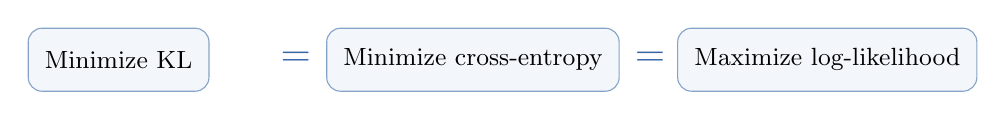
\begin{tikzpicture}[
  eq/.style={draw=popblue!60, fill=popblue!6, rounded corners=5pt, minimum height=0.8cm, align=center, font=\small, inner sep=6pt},
]
  \node[eq] (kl) at (-4.5, 0) {Minimize KL};
  \node[eq] (ce) at (0, 0) {Minimize cross-entropy};
  \node[eq] (ml) at (4.5, 0) {Maximize log-likelihood};
  \node[font=\Large\bfseries, popblue] at (-2.25, 0) {$=$};
  \node[font=\Large\bfseries, popblue] at (2.25, 0) {$=$};
\end{tikzpicture}
\end{center}

\vspace{0.15cm}
\begin{center}
\small\textbf{All three are the same optimization problem!}\\
This is why cross-entropy is THE standard loss function in ML.
\end{center}
\end{frame}

% ============================================================
\begin{frame}
\frametitle{Cross-Entropy Loss in Classification}

\small
Multi-class classification with $g$ classes. For observation $i$:
\begin{itemize}\setlength{\itemsep}{1pt}
  \item True label $y_i \in \{1, \ldots, g\}$, one-hot encoded as $\mathbf{d}^{(i)} = (0, \ldots, 1, \ldots, 0)$
  \item Model outputs probability vector $\boldsymbol{\pi}(\mathbf{x}_i \mid \theta) = (\pi_1, \ldots, \pi_g)$
\end{itemize}

\vspace{0.1cm}
The cross-entropy between one-hot $\mathbf{d}^{(i)}$ and model $\boldsymbol{\pi}$:

\vspace{-0.2cm}
$$H(\mathbf{d}^{(i)} \| \boldsymbol{\pi}) = -\sum_{k=1}^g d_k^{(i)} \log \pi_k(\mathbf{x}_i \mid \theta) = -\log \pi_{y_i}(\mathbf{x}_i \mid \theta)$$

\pause
Summing over all observations:
$$\mathcal{R}(\theta) = -\sum_{i=1}^n \log \pi_{y_i}(\mathbf{x}_i \mid \theta) \qquad\textcolor{popblue}{\text{(= negative log-likelihood = log-loss)}}$$

\vspace{0.1cm}
\begin{center}
\fcolorbox{orange1}{orange1!5}{\parbox{11cm}{\centering\small
  \textbf{Cross-entropy loss IS log-loss IS negative log-likelihood.}\\
  Three names for the same thing. Softmax + cross-entropy = the standard recipe.
}}
\end{center}
\end{frame}

% ============================================================
\begin{frame}
\frametitle{Binary Cross-Entropy = Bernoulli Log-Loss}

\small
Binary classification: $y \in \{0, 1\}$, model outputs $\pi(\mathbf{x}) = P(Y{=}1 \mid \mathbf{x})$.

$$L(y, \pi) = -y\log\pi(\mathbf{x}) - (1-y)\log(1 - \pi(\mathbf{x}))$$

This is the cross-entropy between two Bernoulli distributions:
$p = \text{Bern}(y)$ and $q = \text{Bern}(\pi(\mathbf{x}))$.

\vspace{0.3cm}
\begin{center}
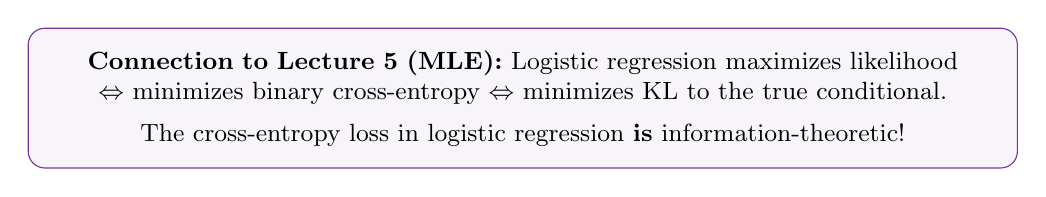
\begin{tikzpicture}
  \node[draw=violet1, fill=violet1!5, rounded corners=6pt, text width=12cm, align=center, inner sep=8pt, font=\small] {
    \textbf{Connection to Lecture~5 (MLE):} Logistic regression maximizes likelihood\\
    $\Leftrightarrow$ minimizes binary cross-entropy $\Leftrightarrow$ minimizes KL to the true conditional.\\[4pt]
    The cross-entropy loss in logistic regression \textbf{is} information-theoretic!
  };
\end{tikzpicture}
\end{center}
\end{frame}

% ============================================================
\begin{frame}
\frametitle{Entropy as Baseline Risk}

\small
What's the best a ``dumb'' model can do? \;Use class frequencies: $\pi_k = n_k / n$.

\vspace{-0.05cm}
The average cross-entropy of this constant model:
\vspace{-0.2cm}
$$\mathcal{R} = -\sum_{k=1}^g \frac{n_k}{n}\log\frac{n_k}{n} = -\sum_k \pi_k \log \pi_k = H(\boldsymbol{\pi})$$

\vspace{-0.1cm}
\begin{center}
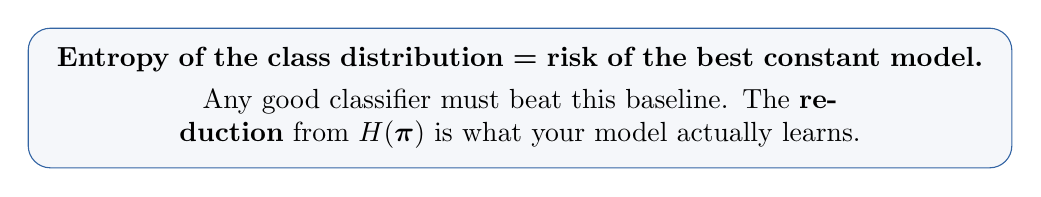
\begin{tikzpicture}
  \node[draw=popblue, fill=popblue!5, rounded corners=8pt, text width=12cm, align=center, inner sep=7pt] {
    \textbf{Entropy of the class distribution = risk of the best constant model.}\\[3pt]
    Any good classifier must beat this baseline.
    The \textbf{reduction} from $H(\boldsymbol{\pi})$ is what your model actually learns.
  };
\end{tikzpicture}
\end{center}

\vspace{0.05cm}
\begin{center}
\renewcommand{\arraystretch}{1.3}
\begin{tabular}{lcc}
  \textbf{Class balance} & \textbf{Baseline entropy} & \textbf{Interpretation} \\
  \hline
  $(0.5, 0.5)$ & 1 bit & Hard (max uncertainty) \\
  $(0.9, 0.1)$ & 0.47 bits & Easy (already pretty sure) \\
  $(0.99, 0.01)$ & 0.08 bits & Trivial (almost deterministic) \\
  \hline
\end{tabular}
\end{center}
\end{frame}

% ============================================================
\section{Forward vs Reverse KL}

\begin{frame}
\begin{center}
\vspace{1cm}
{\LARGE\bfseries\textcolor{popblue}{Forward vs Reverse KL}}\\[15pt]
{\large KL is not symmetric. The direction matters --- a lot.}
\end{center}
\end{frame}

% ============================================================
\begin{frame}
\frametitle{Two Directions, Two Behaviors}

\small
We want to approximate a complex distribution $p$ with a simpler model $q_\phi$.

\vspace{0.2cm}
\begin{columns}[T]
\begin{column}{0.48\textwidth}
\begin{center}
\textcolor{popblue}{\textbf{Forward KL:}} $D_{\text{KL}}(p \| q_\phi)$
\end{center}
\begin{itemize}\setlength{\itemsep}{3pt}
  \item Averages $\log\frac{p}{q_\phi}$ under \textbf{$p$}
  \item Penalizes $q_\phi \approx 0$ where $p > 0$
  \item $q_\phi$ must \textbf{cover all} of $p$'s mass
  \item Behavior: \textbf{mass-covering}
  \item Used in: supervised learning, MLE
\end{itemize}
\end{column}
\begin{column}{0.48\textwidth}
\begin{center}
\textcolor{sampred}{\textbf{Reverse KL:}} $D_{\text{KL}}(q_\phi \| p)$
\end{center}
\begin{itemize}\setlength{\itemsep}{3pt}
  \item Averages $\log\frac{q_\phi}{p}$ under \textbf{$q_\phi$}
  \item Penalizes $q_\phi > 0$ where $p \approx 0$
  \item $q_\phi$ avoids regions where $p$ is small
  \item Behavior: \textbf{mode-seeking}
  \item Used in: variational inference
\end{itemize}
\end{column}
\end{columns}

\vspace{0.2cm}
\begin{center}
\fcolorbox{orange1}{orange1!5}{\parbox{11cm}{\centering\small
  \textbf{Forward KL:} ``I'd rather be too wide than miss anything.''\\
  \textbf{Reverse KL:} ``I'd rather be too narrow than put mass where $p$ doesn't.''
}}
\end{center}
\end{frame}

% ============================================================
\begin{frame}
\frametitle{Forward vs Reverse KL: Fitting a Gaussian to a Bimodal}

\begin{center}
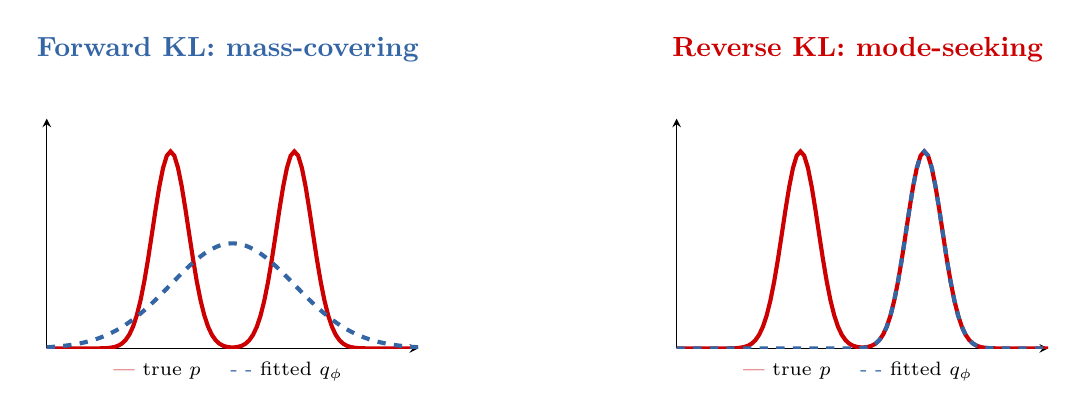
\begin{tikzpicture}
  % --- Forward KL (left) ---
  \begin{scope}[xshift=-4cm]
    \node[font=\bfseries, popblue] at (2.3, 3.8) {Forward KL: mass-covering};
    \begin{axis}[
      at={(0,0)}, width=6.3cm, height=4.5cm,
      xmin=-6, xmax=6, ymin=0, ymax=0.35,
      xtick=\empty, ytick=\empty,
      axis lines=left,
      every axis plot/.append style={line width=1.5pt, samples=100},
    ]
      % Bimodal target
      \addplot[sampred, domain=-6:6] {0.3*exp(-1.5*(x+2)^2) + 0.3*exp(-1.5*(x-2)^2)};
      % Wide Gaussian fit
      \addplot[popblue, dashed, domain=-6:6] {0.16*exp(-x*x/8)};
    \end{axis}
    \node[font=\scriptsize] at (2.3, -0.3) {\textcolor{sampred}{---} true $p$ \quad \textcolor{popblue}{- -} fitted $q_\phi$};
  \end{scope}

  % --- Reverse KL (right) ---
  \begin{scope}[xshift=4cm]
    \node[font=\bfseries, sampred] at (2.3, 3.8) {Reverse KL: mode-seeking};
    \begin{axis}[
      at={(0,0)}, width=6.3cm, height=4.5cm,
      xmin=-6, xmax=6, ymin=0, ymax=0.35,
      xtick=\empty, ytick=\empty,
      axis lines=left,
      every axis plot/.append style={line width=1.5pt, samples=100},
    ]
      % Bimodal target
      \addplot[sampred, domain=-6:6] {0.3*exp(-1.5*(x+2)^2) + 0.3*exp(-1.5*(x-2)^2)};
      % Narrow Gaussian on one mode
      \addplot[popblue, dashed, domain=-6:6] {0.3*exp(-1.5*(x-2)^2)};
    \end{axis}
    \node[font=\scriptsize] at (2.3, -0.3) {\textcolor{sampred}{---} true $p$ \quad \textcolor{popblue}{- -} fitted $q_\phi$};
  \end{scope}
\end{tikzpicture}
\end{center}

\vspace{-0.1cm}
\begin{center}
\small Forward KL produces a \textbf{wide} fit covering both modes (but too flat).\\
Reverse KL locks onto \textbf{one mode} (sharp but misses the other).
\end{center}
\end{frame}

% ============================================================
\begin{frame}
\frametitle{Why Each Direction Is Used}

\small
\begin{center}
\renewcommand{\arraystretch}{1.8}
\begin{tabular}{lll}
  & \textbf{Forward KL:} $D_{\text{KL}}(p \| q_\phi)$ & \textbf{Reverse KL:} $D_{\text{KL}}(q_\phi \| p)$ \\
  \hline
  \textbf{Gradient} & Requires samples from $p$ & Requires samples from $q_\phi$ \\
  \textbf{Works when} & $p$ is the empirical distribution & $p$ is unnormalized (up to $Z$) \\
  \textbf{Use case} & \textcolor{popblue}{Supervised learning (MLE)} & \textcolor{sampred}{Variational inference (VI)} \\
  \textbf{Behavior} & Mass-covering (inclusive) & Mode-seeking (exclusive) \\
  \hline
\end{tabular}
\end{center}

\vspace{0.15cm}
\begin{center}
\fcolorbox{violet1}{violet1!5}{\parbox{11cm}{\centering\small
  \textbf{Forward KL} for supervised learning: we have data from $p$, so we can compute
  the gradient of $D_{\text{KL}}(p \| q_\theta)$ from samples.\\[4pt]
  \textbf{Reverse KL} for variational inference: the posterior $p(\theta \mid \mathbf{X})$ is known
  only up to a constant, but $\nabla_\phi D_{\text{KL}}(q_\phi \| p)$ doesn't need the normalizer.
}}
\end{center}
\end{frame}

% ============================================================
\section{Maximum Entropy Principle}

\begin{frame}
\begin{center}
\vspace{1cm}
{\LARGE\bfseries\textcolor{popblue}{Maximum Entropy Principle}}\\[15pt]
{\large Given partial knowledge, choose the distribution}\\[4pt]
{\large that is \textbf{maximally uncertain} about everything else.}
\end{center}
\end{frame}

% ============================================================
\begin{frame}
\frametitle{The Maximum Entropy Principle (Jaynes, 2003)}

\small
Suppose we know some constraints (e.g., $\mathbb{E}[g_m(X)] = \alpha_m$ for $m = 1, \ldots, M$).
Many distributions satisfy these constraints. Which one should we pick?

\vspace{0.1cm}
\begin{center}
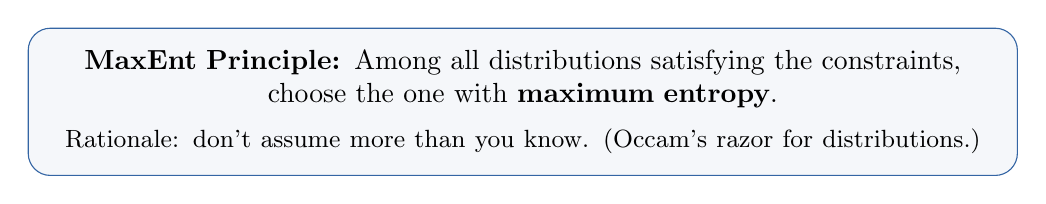
\begin{tikzpicture}
  \node[draw=popblue, fill=popblue!5, rounded corners=8pt, text width=12cm, align=center, inner sep=8pt] {
    \textbf{MaxEnt Principle:} Among all distributions satisfying the constraints,\\
    choose the one with \textbf{maximum entropy}.\\[4pt]
    \small Rationale: don't assume more than you know. (Occam's razor for distributions.)
  };
\end{tikzpicture}
\end{center}

\pause
\vspace{0.05cm}
\textbf{Solution} (Lagrangian):
\vspace{-0.15cm}
$$p^*(x) = \frac{1}{Z}\exp\!\left(\sum_{m=1}^M \lambda_m\, g_m(x)\right) \qquad Z = \sum_x \exp\!\left(\sum_m \lambda_m\, g_m(x)\right)$$

\vspace{-0.05cm}
\begin{center}
\fcolorbox{paramgreen}{paramgreen!5}{\parbox{11cm}{\centering\small
  The MaxEnt distribution is always an \textbf{exponential family} (Gibbs distribution)!\\
  This is no coincidence --- exponential families \textbf{are} the MaxEnt distributions.
}}
\end{center}
\end{frame}

% ============================================================
\begin{frame}
\frametitle{MaxEnt Recovers Familiar Distributions}

\small
Different constraints $\Rightarrow$ different MaxEnt distributions:

\vspace{0.15cm}
\begin{center}
\renewcommand{\arraystretch}{1.6}
\begin{tabular}{lll}
  \textbf{Constraint(s)} & \textbf{MaxEnt distribution} & \textbf{Connection} \\
  \hline
  None (fixed support $\{1,\ldots,g\}$) & Uniform & Max entropy = $\log g$ \\
  $\mathbb{E}[X] = \mu$ (on $\{1,\ldots,g\}$) & Exponential/Gibbs & Biased die \\
  $\mathbb{E}[X] = \mu$, $\text{Var}(X) = \sigma^2$ & \textbf{Gaussian} $N(\mu, \sigma^2)$ & Most common in ML! \\
  $\mathbb{E}[X] = 1/\lambda$ (on $[0, \infty)$) & \textbf{Exponential}$(\lambda)$ & Memoryless \\
  \hline
\end{tabular}
\end{center}

\vspace{0.2cm}
\begin{center}
\fcolorbox{orange1}{orange1!5}{\parbox{11cm}{\centering\small
  \textbf{Why the Gaussian is everywhere in ML:} If you only know the mean and
  variance, the Gaussian is the \textbf{least informative} distribution compatible
  with that knowledge. Any other choice would smuggle in extra assumptions.
}}
\end{center}
\end{frame}

% ============================================================
\begin{frame}
\frametitle{MaxEnt Example: The Biased Die}

\small
A 6-sided die with $\mathbb{E}[X] = 4.8$ (heavier than the usual 3.5). What's the MaxEnt distribution?

\vspace{-0.1cm}
$$p^*(x) = \frac{e^{\lambda x}}{Z(\lambda)}, \qquad Z(\lambda) = \sum_{x=1}^6 e^{\lambda x}, \qquad \sum_{x=1}^6 x\,p^*(x) = 4.8$$

\vspace{-0.25cm}
Solving numerically: $\lambda \approx 0.514$.

\vspace{0.05cm}
\begin{center}
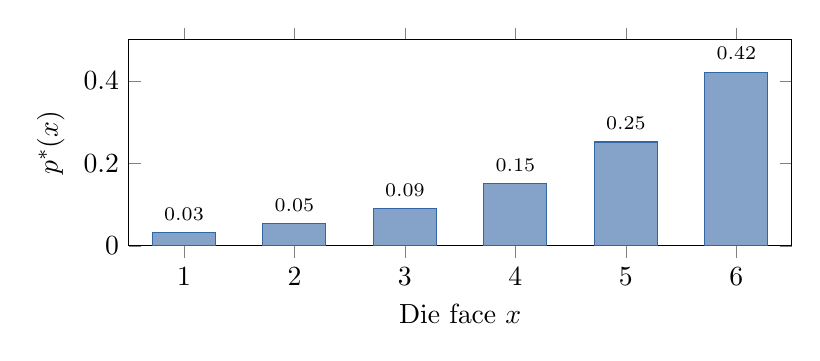
\begin{tikzpicture}
  \begin{axis}[
    width=10cm, height=4.2cm,
    ybar, bar width=0.8cm,
    xlabel={Die face $x$},
    ylabel={$p^*(x)$},
    ymin=0, ymax=0.5,
    xtick={1,2,3,4,5,6},
    nodes near coords,
    every node near coord/.append style={font=\scriptsize, above, yshift=1pt},
    nodes near coords style={/pgf/number format/.cd, fixed, precision=2},
  ]
    \addplot[fill=popblue!60, draw=popblue] coordinates {
      (1, 0.032) (2, 0.054) (3, 0.090) (4, 0.151) (5, 0.252) (6, 0.421)
    };
  \end{axis}
\end{tikzpicture}
\end{center}

\vspace{-0.1cm}
\begin{center}
\small Exponential tilt toward higher faces --- the ``least opinionated'' way to have $\mathbb{E}[X] = 4.8$.
\end{center}
\end{frame}

% ============================================================
\section{Mutual Information}

\begin{frame}
\begin{center}
\vspace{1cm}
{\LARGE\bfseries\textcolor{popblue}{Mutual Information}}\\[15pt]
{\large How much does knowing $X$ tell us about $Y$?}\\[4pt]
{\large A universal measure of dependence.}
\end{center}
\end{frame}

% ============================================================
\begin{frame}
\frametitle{Joint and Conditional Entropy}

\small
\textbf{Joint entropy:} Total uncertainty in $(X, Y)$ together:
$$H(X, Y) = -\sum_{x,y} p(x,y)\,\log p(x,y)$$

\textbf{Conditional entropy:} Remaining uncertainty in $Y$ after observing $X$:
$$H(Y \mid X) = -\sum_{x,y} p(x,y)\,\log p(y \mid x) = \mathbb{E}_X\!\left[H(Y \mid X{=}x)\right]$$

\vspace{0.1cm}
\begin{center}
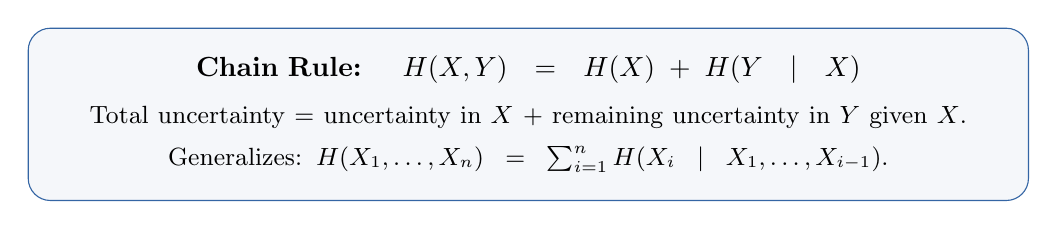
\begin{tikzpicture}
  \node[draw=popblue, fill=popblue!5, rounded corners=8pt, text width=12cm, align=center, inner sep=10pt] {
    \textbf{Chain Rule:} $\;H(X, Y) = H(X) + H(Y \mid X)$\\[6pt]
    \small Total uncertainty = uncertainty in $X$ + remaining uncertainty in $Y$ given $X$.\\[3pt]
    Generalizes: $H(X_1, \ldots, X_n) = \sum_{i=1}^n H(X_i \mid X_1, \ldots, X_{i-1})$.
  };
\end{tikzpicture}
\end{center}

\vspace{0.1cm}
\textbf{Proof:} $\;\log p(x,y) = \log p(x) + \log p(y|x)$. Take $-\mathbb{E}$ of both sides.
\end{frame}

% ============================================================
\begin{frame}
\frametitle{Mutual Information: Definition}

\small
\textbf{Question:} How much does knowing $X$ \textbf{reduce} our uncertainty about $Y$?

\vspace{0.15cm}
\begin{center}
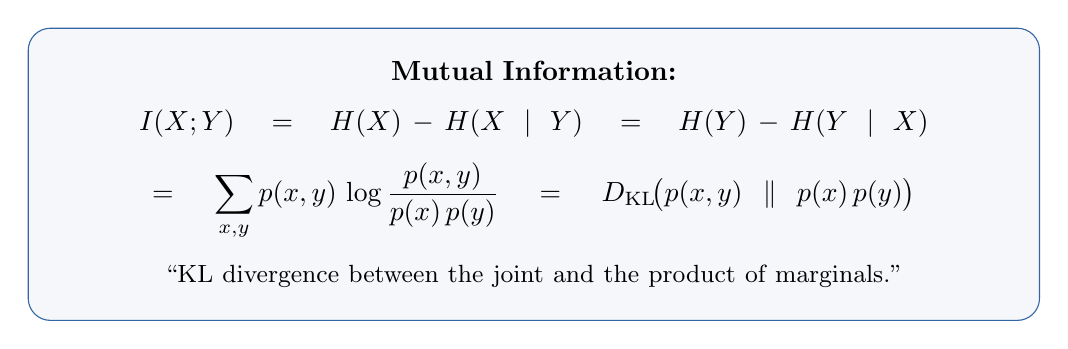
\begin{tikzpicture}
  \node[draw=popblue, fill=popblue!5, rounded corners=8pt, text width=12cm, align=center, inner sep=12pt] {
    \textbf{Mutual Information:}\\[6pt]
    $I(X; Y) \;=\; H(X) - H(X \mid Y) \;=\; H(Y) - H(Y \mid X)$\\[8pt]
    $=\; \displaystyle\sum_{x,y} p(x,y)\,\log\frac{p(x,y)}{p(x)\,p(y)} \;=\; D_{\text{KL}}\!\big(p(x,y) \;\|\; p(x)\,p(y)\big)$\\[8pt]
    \small ``KL divergence between the joint and the product of marginals.''
  };
\end{tikzpicture}
\end{center}

\vspace{0.15cm}
\begin{center}
\fcolorbox{orange1}{orange1!5}{\parbox{11cm}{\centering\small
  MI measures how much the joint distribution \textbf{deviates from independence}.\\
  $I(X;Y) = 0$ iff $X \perp\!\!\!\perp Y$. \;The larger $I(X;Y)$, the more they ``know'' about each other.
}}
\end{center}
\end{frame}

% ============================================================
\begin{frame}
\frametitle{The Information Diagram}

\begin{center}
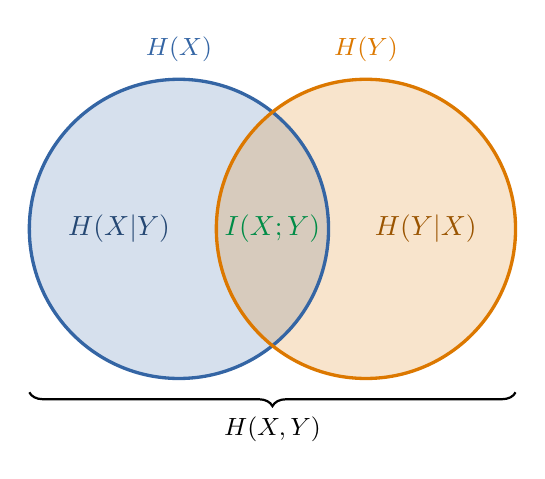
\begin{tikzpicture}[scale=0.95]
  % Circles
  \begin{scope}[opacity=0.2]
    \fill[popblue] (0,0) circle (2);
    \fill[orange1] (2.5,0) circle (2);
  \end{scope}
  \draw[very thick, popblue] (0,0) circle (2);
  \draw[very thick, orange1] (2.5,0) circle (2);

  % Labels inside
  \node[font=\normalsize\bfseries, popblue!70!black] at (-0.8, 0) {$H(X|Y)$};
  \node[font=\normalsize\bfseries, paramgreen] at (1.25, 0) {$I(X;Y)$};
  \node[font=\normalsize\bfseries, orange1!70!black] at (3.3, 0) {$H(Y|X)$};

  % Labels outside
  \node[font=\small\bfseries, popblue] at (0, 2.4) {$H(X)$};
  \node[font=\small\bfseries, orange1] at (2.5, 2.4) {$H(Y)$};

  % Brace for joint
  \draw[decorate, decoration={brace, amplitude=5pt, mirror, raise=5pt}, thick]
    (-2, -2) -- (4.5, -2) node[midway, below, yshift=-10pt, font=\small\bfseries] {$H(X, Y)$};
\end{tikzpicture}
\end{center}

\vspace{0.05cm}
\begin{center}
\small
$I(X;Y) = H(X) + H(Y) - H(X,Y)$ \;---\; the overlap = shared information.
\end{center}
\end{frame}

% ============================================================
\begin{frame}
\frametitle{Properties of Mutual Information}

\vspace{-0.1cm}
\begin{center}
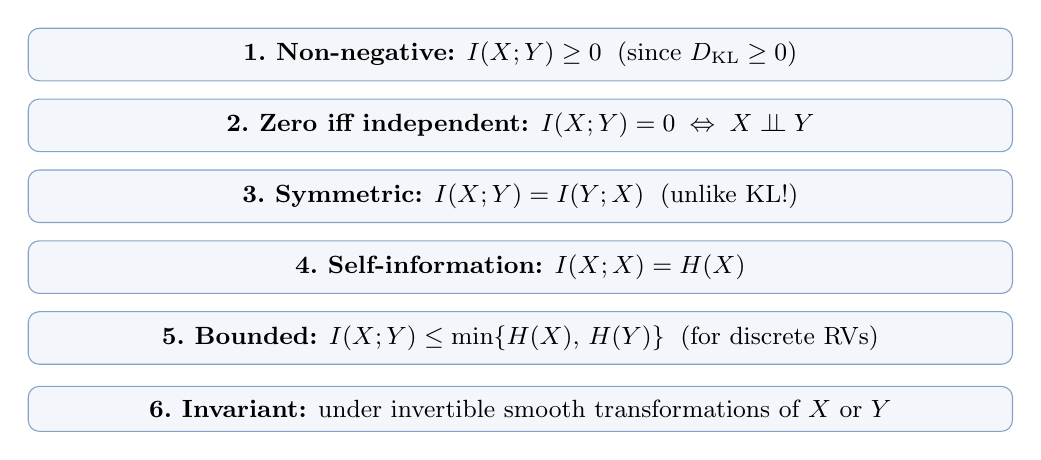
\begin{tikzpicture}[
  pbox/.style={draw=popblue!60, fill=popblue!6, rounded corners=4pt, minimum width=12.5cm, align=left, inner sep=5pt, font=\small}
]
  \node[pbox] at (0, 2.4)  {\textbf{1.~Non-negative:} $I(X;Y) \geq 0$ \;(since $D_{\text{KL}} \geq 0$)};
  \node[pbox] at (0, 1.5)  {\textbf{2.~Zero iff independent:} $I(X;Y) = 0 \;\Leftrightarrow\; X \perp\!\!\!\perp Y$};
  \node[pbox] at (0, 0.6)  {\textbf{3.~Symmetric:} $I(X;Y) = I(Y;X)$ \;(unlike KL!)};
  \node[pbox] at (0, -0.3) {\textbf{4.~Self-information:} $I(X;X) = H(X)$};
  \node[pbox] at (0, -1.2) {\textbf{5.~Bounded:} $I(X;Y) \leq \min\{H(X),\, H(Y)\}$ \;(for discrete RVs)};
  \node[pbox] at (0, -2.1) {\textbf{6.~Invariant:} under invertible smooth transformations of $X$ or $Y$};
\end{tikzpicture}
\end{center}

\vspace{0.15cm}
\begin{center}
\fcolorbox{paramgreen}{paramgreen!5}{\parbox{11cm}{\centering\small
  \textbf{Conditioning reduces entropy (``information can't hurt''):}\\[3pt]
  $H(X \mid Y) \leq H(X)$, with equality iff $X \perp\!\!\!\perp Y$.\\[3pt]
  Proof: $0 \leq I(X;Y) = H(X) - H(X \mid Y)$.
}}
\end{center}
\end{frame}

% ============================================================
\begin{frame}
\frametitle{Worked Example: Computing MI}

\small
\renewcommand{\arraystretch}{1.3}
\begin{columns}[T]
\begin{column}{0.42\textwidth}
\begin{center}
\textbf{Joint distribution} $p(x,y)$:\\[4pt]
\begin{tabular}{c|cccc}
  $X \backslash Y$ & $y_1$ & $y_2$ & $y_3$ & $y_4$ \\
  \hline
  $x_1$ & $\frac{1}{8}$ & $\frac{1}{16}$ & $\frac{1}{32}$ & $\frac{1}{32}$ \\[4pt]
  $x_2$ & $\frac{1}{16}$ & $\frac{1}{8}$ & $\frac{1}{32}$ & $\frac{1}{32}$ \\[4pt]
  $x_3$ & $\frac{1}{16}$ & $\frac{1}{16}$ & $\frac{1}{16}$ & $\frac{1}{16}$ \\[4pt]
  $x_4$ & $\frac{1}{4}$ & $0$ & $0$ & $0$ \\
\end{tabular}
\end{center}
\end{column}
\begin{column}{0.55\textwidth}
\vspace{0.1cm}
\textbf{Marginals:}
\begin{itemize}\setlength{\itemsep}{1pt}
  \item $p_X = (1/4,\; 1/4,\; 1/4,\; 1/4)$
  \item $p_Y = (1/2,\; 1/4,\; 1/8,\; 1/8)$
\end{itemize}

\vspace{0.15cm}
\textbf{Entropies:}
\begin{itemize}\setlength{\itemsep}{1pt}
  \item $H(X) = 2$ bits \quad(uniform over 4)
  \item $H(Y) = 7/4$ bits
  \item $H(X,Y) = 27/8$ bits
\end{itemize}

\vspace{0.15cm}
\textbf{Mutual information:}
$$I(X;Y) = H(X) + H(Y) - H(X,Y)$$
$$= 2 + \tfrac{7}{4} - \tfrac{27}{8} = \boxed{\tfrac{3}{8} \;\text{bits}}$$
\end{column}
\end{columns}
\end{frame}

% ============================================================
\begin{frame}
\frametitle{MI vs Correlation: Why MI Is More General}

\small
\textbf{Pearson correlation} only measures \textbf{linear} dependence. MI captures \textbf{any} dependence.

\vspace{0.2cm}
\begin{center}
\pgfmathsetseed{42}
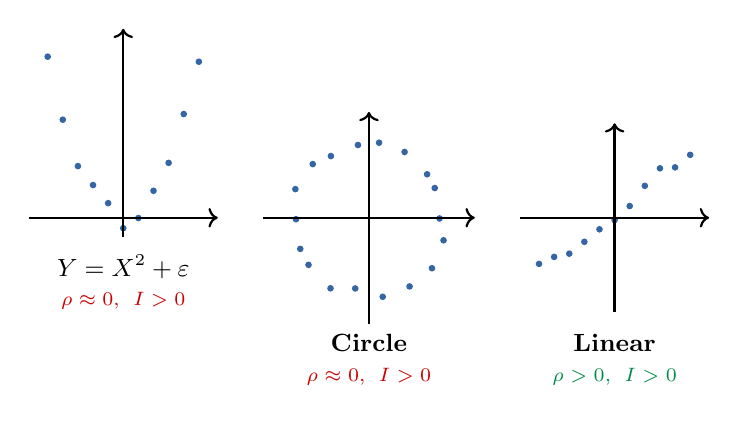
\begin{tikzpicture}[scale=0.48]
  % Parabola
  \begin{scope}[xshift=-6.5cm]
    \foreach \x in {-2,-1.6,...,2} {
      \pgfmathsetmacro{\y}{\x*\x + 0.3*rand}
      \fill[popblue] (\x, \y) circle (2.5pt);
    }
    \draw[thick, ->] (-2.5, 0) -- (2.5, 0);
    \draw[thick, ->] (0, -0.5) -- (0, 5);
    \node[font=\small\bfseries] at (0, -1.3) {$Y = X^2 + \varepsilon$};
    \node[font=\scriptsize, sampred] at (0, -2.2) {$\rho \approx 0$, \;$I > 0$};
  \end{scope}

  % Circle
  \begin{scope}[xshift=0cm]
    \foreach \a in {0,20,...,340} {
      \pgfmathsetmacro{\x}{2*cos(\a) + 0.15*rand}
      \pgfmathsetmacro{\y}{2*sin(\a) + 0.15*rand}
      \fill[popblue] (\x, \y) circle (2.5pt);
    }
    \draw[thick, ->] (-2.8, 0) -- (2.8, 0);
    \draw[thick, ->] (0, -2.8) -- (0, 2.8);
    \node[font=\small\bfseries] at (0, -3.3) {Circle};
    \node[font=\scriptsize, sampred] at (0, -4.2) {$\rho \approx 0$, \;$I > 0$};
  \end{scope}

  % Linear
  \begin{scope}[xshift=6.5cm]
    \foreach \x in {-2,-1.6,...,2} {
      \pgfmathsetmacro{\y}{0.8*\x + 0.4*rand}
      \fill[popblue] (\x, \y) circle (2.5pt);
    }
    \draw[thick, ->] (-2.5, 0) -- (2.5, 0);
    \draw[thick, ->] (0, -2.5) -- (0, 2.5);
    \node[font=\small\bfseries] at (0, -3.3) {Linear};
    \node[font=\scriptsize, paramgreen] at (0, -4.2) {$\rho > 0$, \;$I > 0$};
  \end{scope}
\end{tikzpicture}
\end{center}

\vspace{-0.1cm}
\begin{center}
\fcolorbox{orange1}{orange1!5}{\parbox{11cm}{\centering\small
  \textbf{Correlation = 0 does NOT mean independence.}
  MI detects \textbf{any} dependence --- linear, nonlinear, or otherwise.
}}
\end{center}
\end{frame}

% ============================================================
\begin{frame}
\frametitle{MI for Correlated Gaussians}

\small
For $(X, Y) \sim N\!\left(\mathbf{0},\; \begin{pmatrix}\sigma^2 & \rho\sigma^2\\ \rho\sigma^2 & \sigma^2\end{pmatrix}\right)$:

$$I(X; Y) = -\frac{1}{2}\log_2(1 - \rho^2)$$

\begin{center}
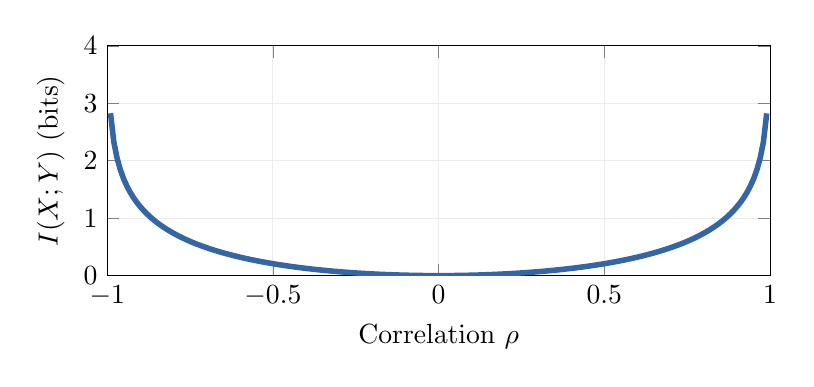
\begin{tikzpicture}
  \begin{axis}[
    width=10cm, height=4.5cm,
    xlabel={Correlation $\rho$},
    ylabel={$I(X;Y)$ (bits)},
    domain=-0.99:0.99,
    xmin=-1, xmax=1,
    ymin=0, ymax=4,
    grid=major, grid style={gray!15},
    xtick={-1, -0.5, 0, 0.5, 1},
    every axis plot/.append style={line width=2pt},
  ]
    \addplot[popblue, samples=200] {-0.5*ln(1 - x*x)/ln(2)};
  \end{axis}
\end{tikzpicture}
\end{center}

\vspace{-0.1cm}
\begin{center}
\small $\rho = 0 \Rightarrow I = 0$ (Gaussian: uncorrelated $=$ independent).\\
$|\rho| \to 1 \Rightarrow I \to \infty$ (perfect linear dependence).
\end{center}
\end{frame}

% ============================================================
\begin{frame}
\frametitle{MI in ML: Information Gain in Decision Trees}

\small
At each node of a decision tree, we pick the feature that \textbf{maximizes information gain}:

$$\text{IG}(Y; X_j) = H(Y) - H(Y \mid X_j) = I(Y; X_j)$$

\vspace{-0.3cm}
\begin{center}
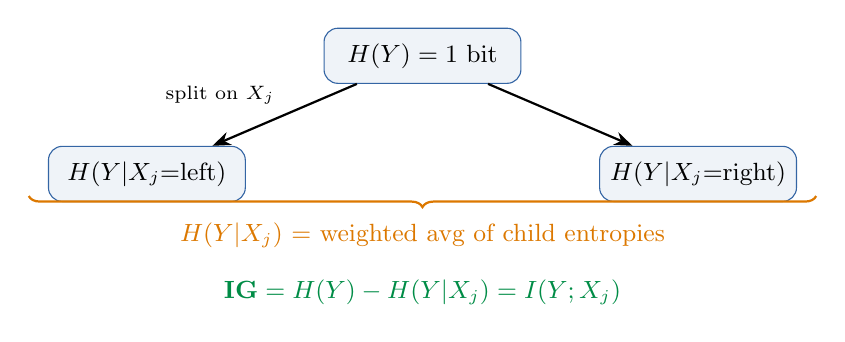
\begin{tikzpicture}[
  nd/.style={draw=popblue, fill=popblue!8, rounded corners=5pt, minimum width=2.5cm, minimum height=0.7cm, align=center, font=\small},
  arr/.style={-{Stealth}, thick},
]
  \node[nd] (root) at (0, 0) {$H(Y) = 1$ bit};
  \node[nd] (l) at (-3.5, -1.5) {$H(Y|X_j{=}\text{left})$};
  \node[nd] (r) at (3.5, -1.5) {$H(Y|X_j{=}\text{right})$};
  \draw[arr] (root) -- node[above left, font=\scriptsize] {split on $X_j$} (l);
  \draw[arr] (root) -- (r);
  \draw[decorate, decoration={brace, amplitude=4pt, raise=8pt, mirror}, thick, orange1]
    (-5, -1.5) -- (5, -1.5) node[midway, below, yshift=-14pt, font=\small] {$H(Y|X_j)$ = weighted avg of child entropies};

  \node[font=\small\bfseries, paramgreen] at (0, -3) {$\text{IG} = H(Y) - H(Y|X_j) = I(Y; X_j)$};
\end{tikzpicture}
\end{center}

\vspace{-0.2cm}
\begin{center}
\fcolorbox{popblue}{popblue!5}{\parbox{11cm}{\centering\small
  \textbf{Split on the feature with highest MI with the target.}\\
  Exactly the criterion in ID3, C4.5, CART (entropy impurity).
  Feature selection: rank features by $I(X_j; Y)$, pick top ones.
}}
\end{center}
\end{frame}

% ============================================================
\section{Summary}

\begin{frame}
\frametitle{The Information Theory Toolbox for ML}

\vspace{-0.2cm}
\begin{center}
\footnotesize
\renewcommand{\arraystretch}{1.5}
\begin{tabular}{lll}
  \textbf{Concept} & \textbf{Formula} & \textbf{ML Role} \\
  \hline
  Entropy $H(p)$ & $-\sum p\log p$ & Baseline risk, impurity \\
  Cross-entropy $H(p\|q)$ & $-\sum p\log q$ & \textbf{Loss function} (log-loss) \\
  KL divergence $D_{\text{KL}}$ & $\sum p\log\frac{p}{q}$ & MLE, variational inference \\
  Mutual info $I(X;Y)$ & $D_{\text{KL}}(p_{xy}\|p_x p_y)$ & Feature selection, info gain \\
  Forward KL & $D_{\text{KL}}(p\|q_\theta)$ & Supervised learning \\
  Reverse KL & $D_{\text{KL}}(q_\phi\|p)$ & Variational inference \\
  MaxEnt & $\arg\max H$ s.t.\ constraints & Gaussian, exp family \\
  \hline
\end{tabular}
\end{center}

\vspace{0.1cm}
\begin{center}
\fcolorbox{paramgreen}{paramgreen!5}{\parbox{11cm}{\centering\small
  \textbf{Key takeaway:} Information theory is not just ``theory'' --- it directly gives us
  the loss functions, optimization objectives, and model selection criteria we use every day in ML.
}}
\end{center}
\end{frame}

% ============================================================
\begin{frame}
\frametitle{Homework}

\begin{enumerate}\setlength{\itemsep}{2pt}
  \item Show that minimizing cross-entropy $H(\hat{p} \| q_\theta)$ over training data
    is equivalent to maximizing the log-likelihood.

  \item For the joint distribution in the worked example,
    verify $I(X;Y) = H(X) - H(X|Y) = H(Y) - H(Y|X) = 3/8$ bits.

  \item Binary classification with $P(Y{=}1) = 0.7$.
    \begin{itemize}\setlength{\itemsep}{0pt}
      \item[(a)] Compute $H(Y)$.
      \item[(b)] If $H(Y|X) = 0.5$ bits after observing feature $X$, what is $I(X;Y)$?
      \item[(c)] Compare: feature $X'$ with $I(X';Y) = 0.01$ bits. Which is more useful?
    \end{itemize}

  \item Explain intuitively why forward KL is ``mass-covering'' and reverse KL is ``mode-seeking.''
\end{enumerate}
\end{frame}

% ============================================================
\begin{frame}
\begin{center}
  {\Huge\bfseries\textcolor{popblue}{Questions?}}
\end{center}
\end{frame}

\end{document}
